\chapter{Experiments}

In this chapter we describe various experiments that were performed to evaluate the effectiveness and necessity of optimizations described in the previous chapter.
These experiments compare the time required to solve particular instances across two or more variants.
Each variant can be either a modification to the instance itself (by changing the way it is generated), or the instance can be unchanged but rather the behavior of the SAT solver itself is modified.

\section{Methodology}
Since the running time of a SAT solver is not deterministic it is not enough to simply perform a single run for every instance.
In fact, given the same instance and the same SAT solver the running time can differ significantly, even by several orders of magnitude.
Multiple samples therefore have to be gathered and sound statistical methods used to discover patterns in this noisy data.

\subsubsection{Sampling procedure}
To counter the high variability in time even for one instance we will solve each instance several times.

Additionally, not all instances for particular parameters (such as number of rounds) are equally hard.
For example, reduced hash functions with significantly lower number of rounds than the full hash function do not behave sufficiently as random functions.
Some output digests might be significantly less likely to be produced than other, or might not be even be possible.
When we are performing a partial preimage attack by fixing several digest bits to be equal to a reference digest (obtained by first hashing a random message) some instances might have fewer solutions than others and be therefore harder.

For this reason we also perform all such experiments on multiple instances that have identical parameters but the random reference messages are independently generated.

\subsubsection{Censoring}
Sometimes we might obtain an instance that takes very long time to solve.
To ensure that experiments finish in a reasonable time it is common to enforce a time limit and abort all computations that exceed it.
Since in such cases we can not know the true running time we must discard these aborted measurements.

Data sets with such discarded measurements are called \emph{censored}.
They make statistical analysis complicated if not impossible, since even trivial statistics such as mean can not be computed without knowing the true censored values.

For this reason we avoided censoring in our experiments.
While we did have a time limit in place, all experiments that contained censored runs were discarded and not considered for analysis.
To obtain valid experiments we either increased the time limit or reduced some of the parameters (such as number of rounds or length of the preimage) until we got a configuration that finished without any censoring.

\subsubsection{Statistical analysis}
For plots of solving time versus some parameter of the instance the most useful statistic is the mean.
It shows the general trend in behavior and the rate with which the time increases.
However it is by itself unreliable since the random variability can affect it significantly.

For this reason we also include $95\%$ confidence intervals in our plots.
By performing more and more repetitions and obtaining more samples we can reduce the size of those intervals and obtain reliable results.

It is important to note that standard techniques for computing means and confidence intervals require either normal distribution of the data, or at least some knowledge about the distribution.
With SAT solving times we have neither -- although the solving times for some cryptographic instances have been shown \cite{bard2007efficient} to have a log-normal distribution we would still have to verify this assumption for our data sets.

Instead we use the $BC_a$ bootstrap procedure \cite{diciccio1996bootstrap} for calculating means and confidence intervals that does not require any knowledge or assumptions about the distribution.

To evaluate the effect of some optimization on the running time we need a statistical procedure to decide if there is a significant difference in the running time distribution or if all differences can be attributed to chance.
Since experiments can have varying parameters (such as number of rounds) and for each parameter combination we run multiple independent samples a pairwise sample comparison is required.
There are several such procedures, such as the Student's t-test or the Tukey's test.

However, both of those make assumptions about the underlying distributions which are not met in our case.
For that reason we use the rather less known \emph{Games-Howell} procedure \cite{games1976pairwise} which does not require these assumptions.

Both used procedures are implemented by the \emph{R} statistical computing language \cite{rteam2013}.
Availability of implementations was also a factor when deciding on methodology -- using a tested implementation greatly reduces the chance of errors.

\section{Expression encoding evaluation}
\label{sec:expression-encoding-eval}
In this section we discuss the effect of expression encoding optimizations described in section \ref{sec:expression-encoding}.
We performed this experiment on two hash functions, the \emph{SHA-1} and \emph{SHA-3}.

\subsection{SHA-1 analysis}
We evaluated the effectiveness of this optimization on preimage attacks on \emph{SHA-1} using the unmodified Tseitin encoding and using the \emph{Espresso} optimizer on both the \emph{choice} and \emph{majority} round functions.
We measured the running time of finding an $8$-bit preimage for $32$-bit input message.
The preimage bits were obtained by hashing random messages to ensure a solution would exist even for instances with reduced number of rounds.
We repeated the experiment multiple times for a total of $5670$ samples for each variant.
 
Figure \ref{fig:opt-sha1-cmp-espresso} shows the mean running times for both instances without optimizations and for ones using \emph{Espresso} minimization.
As we can see the effect of this optimization is quite small and the running times appear to be identical.

%> posthocTGH(y=raw[raw$rounds>20,]$time, x=raw[raw$rounds>20,]$label, method='games-howell')
%          n means variances
%s1espr 4200   2.5       7.4
%s1none 4200   2.6       7.4
%
%                t   df    p
%s1espr:s1none 1.6 8398 0.12

Using the Games-Howell post hoc test on instances with more than $20$ rounds (to reduce the effect of randomness when measuring very short time intervals) we do obtain a mean time improvement of $t=1.6$ seconds however at a fairly high significance level of $p=0.12$ which does not give us enough evidence to reject the hypothesis that this optimization leads to no improvement.

\subsection{SHA-3 analysis} 
\label{sec:sha3-espresso}

%> posthocTGH(y=raw[raw$rounds>12,]$time, x=raw[raw$rounds>12,]$label, method='games-howell')
%          n means variances
%s3esno  949   7.4        50
%s3esxor 949   8.2        54
%s3nono  949   7.5        45
%s3noxor 949   8.5        49
%
%                   t   df      p
%s3esno:s3esxor  2.56 1892 0.0521
%s3esno:s3nono   0.52 1891 0.9540
%s3esno:s3noxor  3.63 1896 0.0016
%s3esxor:s3nono  2.11 1878 0.1499
%s3esxor:s3noxor 0.98 1891 0.7581
%s3nono:s3noxor  3.21 1892 0.0075
\begin{figure*}
\centering \begin{tabular}{ccrccrr}
\multicolumn{2}{c}{\textbf{Optimizations}} & \multicolumn{1}{c}{\textbf{Time}} & \multicolumn{2}{c}{\textbf{Optimizations}} & \multicolumn{2}{c}{\textbf{Time}} \\
\textbf{$\chi$ step} & \textbf{$\theta$ step} & \multicolumn{1}{c}{\textbf{Mean}} & \textbf{$\chi$ step} & \textbf{$\theta$ step} & \textbf{t} & \textbf{p}\\ \hline
\xmark & \xmark & $7.5$ & \xmark & \cmark & $3.21$ & $<0.01$ \\
& & & \cmark & \xmark & $0.52$ & $0.95$ \\
& & & \cmark & \cmark & $2.11$ & $0.15$ \\ \hline
\xmark & \cmark & $8.5$ & \cmark & \xmark & $3.63$ & $<0.01$ \\
& & & \cmark & \cmark & $0.98$ & $0.75$ \\ \hline
\cmark & \xmark & $7.4$ & \cmark & \cmark & $2.56$ & $0.05$ \\ \hline
\cmark & \cmark & $8.2$ & \\
\end{tabular}
\caption{Pairwise comparison of four \emph{SHA-3-512} optimization combinations using the Games-Howell procedure. Only measurements for more than $12$ rounds were used to avoid randomness in timing, for a total of $n=949$ samples per strategy.}
\label{tbl:gh-sha3-opts}
\end{figure*}

We performed a similar experiment for the \emph{SHA-3} hash function, finding an $8$-bit preimage on $32$-bit message where the preimage bits again came from randomly generated messages.
We considered two possible optimizations in the round function and tested four variants -- all combinations of turning on or off these two optimizations.
A total of $2000$ samples was collected for each variant.

The first optimization was minimizing the expression $x \oplus (\overline{y} \land z)$ in the $\chi$ step, which is used to fill the $5\times 5$ state matrix $S$ in each round.

The second optimization was in the $\theta$ step, where the $C$ vector is filled using an exclusive or of five different values.
Without optimization this leads to four extra variables and 16 extra clauses.
Using the Espresso minimization will lead to 32 clauses but only one extra variable.

Using the Games-Howell procedure again we obtain the pairwise comparison shown in figure \ref{tbl:gh-sha3-opts}.

We can see that the \emph{xor} optimization -- which reduces the number of variables but requires twice as many clauses -- in fact leads to higher solving time (mean difference $t=3.21$) at significance level of $p < 0.01$.
Thus the default behavior is more efficient.
On the other hand, from the high p-value of $0.75$ we can't reject the hypothesis that optimizing the $\chi$ step makes no difference at all.

\subsection{Discussion}
Even with large number of samples to eliminate the intrinsic randomness in SAT solving times we were unable to reject hypotheses that the tested optimizations do not lead to an improvement.
From this we conclude that they do not provide significant benefits.

While our library provides this optimization feature to users as we saw in our measurements it is not necessary to use it.
Therefore minimal changes to existing, off-the-shelf implementations of hash functions (without the need to identify expressions with non-optimal Tseitin representation) are sufficient to match the hand-optimized instances such as in \cite{nossum2012sat}.

\begin{figure*}	
\centering 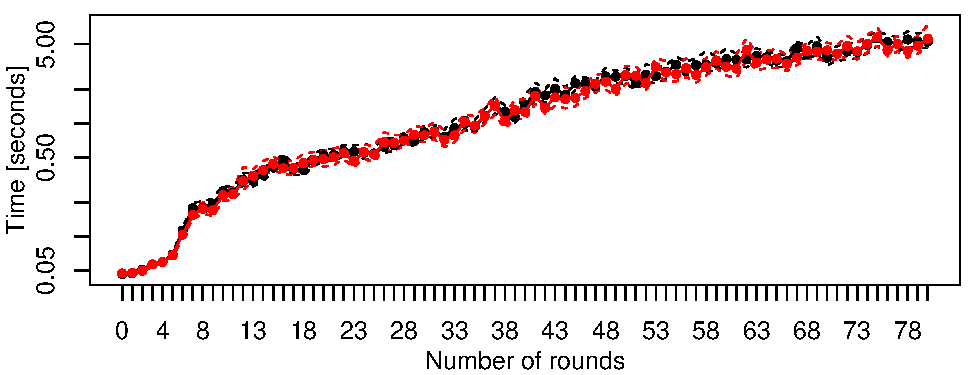
\includegraphics{figures/opt-sha1/sha1-32bit-8bitref-cmp-espresso.pdf}
\caption{Mean running time and 95\% confidence intervals for $8$-bit preimage attack on \emph{SHA-1} without optimizations (black) and using Espresso minimization for rounds functions (red).}
\label{fig:opt-sha1-cmp-espresso}
\end{figure*}

\begin{figure*}
\centering 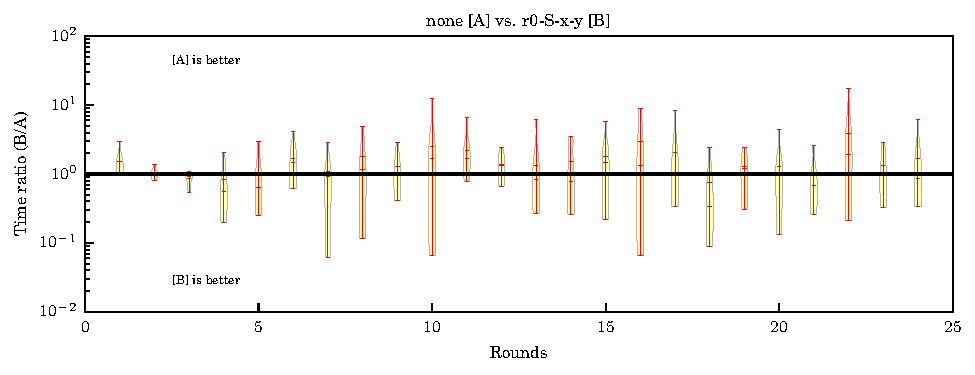
\includegraphics{figures/bo-ex1/ratio-time-none-r0sxy.pdf}
\caption{Violin plot showing the ratios distribution of solving time for the \emph{none} and \emph{r0-S-x-y} strategies.}
\label{fig:bo-ratio-time-none-r0sxy}
\end{figure*}

\begin{figure*}
\centering 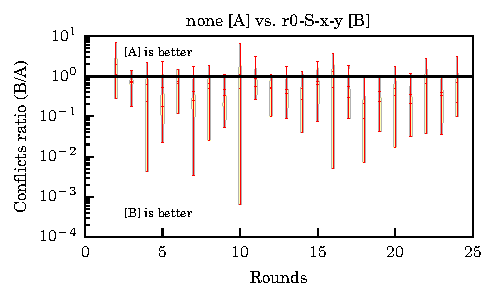
\includegraphics{figures/bo-ex1/ratio-confl-none-r0sxy.pdf}
\caption{Violin plot showing the ratios distribution of number of conflicts for the \emph{none} and \emph{r0-S-x-y} strategies.}
\label{fig:bo-ratio-confl-none-r0sxy}
\end{figure*}

\section{Branching order evaluation}
For branching order optimization described in section \ref{sec:branching-order} we used the \emph{SHA-3} hash function for evaluation.

\subsection{SHA-3 analysis}
For \emph{SHA-3-512} we tested various branching orders on $8$-bit reference preimage attack with number of rounds ranging from $1$ to $24$ (the maximum for this hash function).
For every number of rounds 10 different instances were generated and each was solved 10 times, for a total of 100 samples per round per strategy.
We compared the following branching order strategies:

\textbf{\emph{none}}: No branching order was specified. This is the default unmodified MiniSat behavior.

\textbf{\emph{r0-S-x-y}}: The $S$ matrix from the first round is branched on first, in column-major order.

\textbf{\emph{r0-S-y-x}}: Same as previous one, but in row-major order.

\textbf{\emph{rlast-S-x-y}} and \textbf{\emph{rlast-S-y-x-}}: Same as previous two, but the $S$ matrix from the last round is used instead.	

The figures \ref{fig:bo-ratio-time-none-r0sxy} and \ref{fig:bo-ratio-confl-none-r0sxy} show \emph{violin plots} of the distribution of ratios of the solving time and the number of conflicts.
Each \emph{violin} also show the mean, median and extreme values.

From these plots we see that while the ratios for the number of conflict are mostly below 1 (meaning that the \emph{r0-S-x-y} strategy leads to fewer conflicts), the time ratios are often higher than 1.

%> posthocTGH(y=confl[confl$rounds>12,]$time, x=confl[confl$rounds>12,]$label, method='games-howell')
%              n means variances
%none        480   731    330234
%r0-S-x-y    480   250     51256
%r0-S-y-x    480   250     51256
%rlast-S-x-y 480   731    330234
%rlast-S-y-x 480   731    330234
%
%                         t  df       p
%none:r0-S-x-y           17 624 1.7e-10
%none:r0-S-y-x           17 624 1.7e-10
%none:rlast-S-x-y         0 958 1.0e+00
%none:rlast-S-y-x         0 958 1.0e+00
%r0-S-x-y:r0-S-y-x        0 958 1.0e+00
%r0-S-x-y:rlast-S-x-y    17 624 1.7e-10
%r0-S-x-y:rlast-S-y-x    17 624 1.7e-10
%r0-S-y-x:rlast-S-x-y    17 624 1.7e-10
%r0-S-y-x:rlast-S-y-x    17 624 1.7e-10
%rlast-S-x-y:rlast-S-y-x  0 958 1.0e+00
%> posthocTGH(y=time[time$rounds>12,]$time, x=time[time$rounds>12,]$label, method='games-howell')
%              n means variances
%none        480   7.8        35
%r0-S-x-y    480   7.5        39
%r0-S-y-x    480   7.5        38
%rlast-S-x-y 480   7.8        36
%rlast-S-y-x 480   7.8        35
%
%                            t  df    p
%none:r0-S-x-y           0.647 956 0.97
%none:r0-S-y-x           0.576 956 0.98
%none:rlast-S-x-y        0.185 958 1.00
%none:rlast-S-y-x        0.032 958 1.00
%r0-S-x-y:r0-S-y-x       0.071 958 1.00
%r0-S-x-y:rlast-S-x-y    0.826 956 0.92
%r0-S-x-y:rlast-S-y-x    0.680 956 0.96
%r0-S-y-x:rlast-S-x-y    0.755 957 0.94
%r0-S-y-x:rlast-S-y-x    0.609 956 0.97
%rlast-S-x-y:rlast-S-y-x 0.153 958 1.00
\begin{figure*}
\centering \begin{tabular}{lrrlrrrr}
\textbf{Strategy} & \textbf{Time} & \textbf{Conflicts} & \textbf{Strategy} & \multicolumn{2}{c}{\textbf{Time}} & \multicolumn{2}{c}{\textbf{Conflicts}} \\
& \multicolumn{2}{c}{\textbf{Mean}} & & \textbf{t} & \textbf{p} & \textbf{t} & \textbf{p} \\ \hline
\emph{none} & $7.8$ & $731$ & \emph{r0-S-x-y} & $0.65$ & $0.97$ & $17$ & $<0.01$ \\
& & & \emph{r0-S-y-x} & $0.58$ & $0.98$ & $17$ & $<0.01$ \\
& & & \emph{rlast-S-x-y} & $0.18$ & $>0.99$ & $958$ & $>0.99$ \\
& & & \emph{rlast-S-y-x} & $0.03$ & $>0.99$ & $958$ & $>0.99$ \\ \hline
\emph{r0-S-x-y} & $7.5$ & $250$ & \emph{r0-S-y-x} & $0.07$ & $>0.99$ & $0$ & $<0.01$ \\	
& & & \emph{rlast-S-x-y} & $0.83$ & $0.92$ & $17$ & $<0.01$ \\
& & & \emph{rlast-S-y-x} & $0.68$ & $0.96$ & $17$ & $<0.01$ \\ \hline
\emph{r0-S-y-x} & $7.5$ & $250$ & \emph{rlast-S-x-y} & $0.76$ & $0.94$ & $17$ & $<0.01$ \\
& & & \emph{rlast-y-x} & $0.60$ & $0.97$ & $17$ & $<0.01$ \\ \hline
\emph{r0-last-x-y} & $7.8$ & $731$ & \emph{rlast-S-y-x} & $0.15$ & $>0.99$ & $0$ & $>0.99$ \\ \hline
\emph{r0-last-y-x} & $7.8$ & $731$ & & & & &  \\
\end{tabular}
\caption{Pairwise comparison of various branching order strategies for \emph{SHA-3-512} using the Games-Howell procedure. Only measurements for more than $12$ rounds were used to avoid randomness in timing for a total of $n=480$ samples per strategy.}
\label{tbl:gh-sha3-bos}
\end{figure*}

The Games-Howell procedure (figure \ref{tbl:gh-sha3-bos}) confirms these findings, with the mean difference for number of conflicts between the \emph{none} and \emph{r0-S-x-y} strategies of $t = 17$ at significance level $p < 0.01$.
However, for the solving time the high p-value does not let us reject the hypothesis that any difference is due to chance.
Note that once again only samples for more than $12$ rounds were included to avoid the strong effect of randomness for instances that solve in very short time.

The \emph{r0-S-y-x} strategy behaves the same as \emph{r0-S-x-y} -- the number of conflicts for every instance is identical and the differences in time are negligible.
On the other hand the strategies starting with the last round's $S$ matrix lead to the same behavior as not providing any branch ordering at all (the \emph{none} strategy).

Similar experiments were performed with the auxiliary vectors and matrices $B, C$ and $D$ with the same results -- enforcing branching order did not lead to better solving times.

\subsection{Discussion}

The fact that these branching order do not change the solving time significantly must mean that either their choice does not lead to any forced assignments and conflicts (which is highly unlikely) or that the default MiniSat heuristic is also picking them for branching first.
The second case means that this optimization is unnecessary and that the default SAT solver heuristic is sufficient in this case.